\documentclass[conference]{IEEEtran}
\IEEEoverridecommandlockouts
% The preceding line is only needed to identify funding in the first footnote. If that is unneeded, please comment it out.
\usepackage{cite}
\usepackage{amsmath,amssymb,amsfonts}
\usepackage{algorithmic}
\usepackage{graphicx}
\usepackage{textcomp}
\usepackage{xcolor}
\usepackage{hyperref}
\usepackage{float}
\def\BibTeX{{\rm B\kern-.05em{\sc i\kern-.025em b}\kern-.08em
    T\kern-.1667em\lower.7ex\hbox{E}\kern-.125emX}}
\begin{document}

\title{Timetabling Problem}

\author{\IEEEauthorblockN{Guilherme Silva (201603647)}
\IEEEauthorblockA{\textit{IART} \\
\textit{FEUP}\\
Porto, Portugal \\
up201603647@fe.up.pt}
\and
\IEEEauthorblockN{Miguel Duarte (201606298)}
\IEEEauthorblockA{\textit{IART} \\
\textit{FEUP}\\
Porto, Portugal \\
up201606298@fe.up.pt}
\and
\IEEEauthorblockN{Rui Alves (201606746)}
\IEEEauthorblockA{\textit{IART} \\
\textit{FEUP}\\
Porto, Portugal \\
up201606746@fe.up.pt}
}

\maketitle

\begin{abstract}

The aim of this paper is to implement and compare Artificial Intelligence algorithms for solving a \textit{Timetabling Problem}, in which a set of events need to be scheduled into rooms at certain time slots, given certain restrictions. The objective is to achieve the best possible allocation efficiently, enforcing the \textit{Hard Constraints} and maximizing the number of \textit{Soft Constraints} verified.
The problem will be described and then formulated as an \textit{Optimization Problem}, together with some discussion on the reasoning behind some of the decisions taken during this process.
Several algorithms will be investigated, along with testing them in different configurations of these types of problems, which have varying difficulty and complexity. Both the efficiency in reaching a solution and its optimality will be taken into account in the pursuit for the optimal algorithm.
\end{abstract}

\begin{IEEEkeywords}
Artificial Intelligence, Scheduling Problems, Optimization Problems, Optimization Algorithms, Hill Climbing, Simulated Annealing, Genetic Algorithms, Python3, pypy
\end{IEEEkeywords}

\section{Introduction}

The problem that is the subject of study in this paper (a \textit{Timetabling Problem}) will be approached with several different \textit{Optimization Algorithms}, implemented in \textit{Python3}, in order to conclude what is the best approach for solving it using \textit{Artificial Intelligence Algorithms}.

Firstly, the problem will be described in further detail, ensuring that all non-formal aspects of it are well documented. Secondly, it will be formulated as an \textit{Optimization Problem}, with the approach taken in doing so being illustrated in increased depth, providing reasoning for the decisions taken. Thirdly, a research on related work on this topic will be presented, giving some insight on the problem from other points of view. Then, the project implementation details will be discussed and the optimization algorithms will be explained in detail. Furthermore, the developed experiments will be presented, along with the obtained results.

Finally, a section will cover the main conclusions obtained in the project development, as well as elaborating on what can be done to further develop work related to this topic.

\section{Problem Description}

The \textit{Timetabling Problem} that is subject of study in this project was designed by Ben Paechter, a professor in the Edinburgh University and consists in a reduction of a typical university course timetabling problem.

In this problem, a given set of events has to be scheduled into one hour time slots, over the course of 5 days with 9 hours of active time each (totaling 45 time slots). The events take place in a given set of rooms, each with its own size (number of sets), and require certain features (which may or not be available in a room). The students attend a given set of these events. 

The goal is to assign the events to the available rooms, in a such a way that the given \textbf{Hard Constraints} are respected and that the given \textbf{Soft Constraints} are verified as much as possible. A given proposed solution is assigned a certain penalty based on the constraints that are not being respected. The optimal solution (if existent for a given input) has a penalty of 0.

\subsection{Hard Constraints}

The hard constraints must be respected by any solution. If any of them are not respected, a penalty of Infinity is assigned to the solution.

They are the following:

\begin{itemize}
    \item Only one event can take place in a room at any given time slot
    \item A student can only attend one event at the same time
    \item The room must be big enough for all the students that are attending the event
    \item The room must satisfy all the features that are required for the event
\end{itemize}

\subsection{Soft Constraints}

The soft constraints are used to evaluate the quality of a valid solution (a solution that respects all the hard constraints), assigning a penalty based on that quality. The assigned penalty is equal to the sum of the penalties of each soft constraint constraint violation.

They are the following: 

\begin{itemize}
    \item A student attends an event in the last time slot of the day. For each student that only attends an event in a given day, a penalty of value 1 is assigned.
    \item A student attends more than two events consecutively. For each consecutively attended event (above 2), a penalty of value 1 is assigned (e.g. 3 consecutive events result in a penalty of 1, 4 consecutive events result in a penalty of 2, an so on). 
    \item A student has a single class on a day. For each student that attends only one event in a given day, a penalty of 1 is assigned.
\end{itemize}

\section{Problem Formulation}

The given scheduling problem can be formulated as an \textit{Optimization Problem}, in which the goal is to minimize the penalty of the given solution.

\subsection{Solution Representation}

The optimization problem will be solved using different algorithms, such as \textit{Hill Climbing} and \textit{Genetic Algorithms}. Thus, the solution representation should provide efficient methods for evaluation and manipulation (mutations and cross-over).

For this reason, a solution consists in an array with size equal to the number of events to be allocated. The array's index represents the id of the event. The array value in that index contains a number representing the \textbf{time slot identifier}. This number consists in the sum between the room number (between 0 and the number of available rooms - 1) and the time slot number (between 0 and 44) multiplied by the number of available rooms. Example:

Assuming that there are 2 days with 3 time slots each (6 time slots total). There are 5 different rooms. There are 3 events to be allocated and a possible solution is represented by the array [8, 25, 16]. The solution is interpreted in the following way:

\begin{itemize}
    \item Event 0 was assigned time slot identifier 8. The time slot number is equal to 8 divided by the number of available rooms (8 / 5 = 1). The room number is equal to the remainder of 8 divided by the number of available rooms (8 \% 5 = 3).
    \item Event 1 was assigned time slot identifier 25. The time slot number is equal to 25 divided by the number of available rooms (25 / 5 = 5). The room number is equal to the remainder of 25 divided by the number of available rooms (25 \% 5 = 0).
    \item Event 2 was assigned time slot identifier 16. The time slot number is equal to 16 divided by the number of available rooms (16 / 5 = 3). The room number is equal to the remainder of 16 divided by the number of available rooms (16 \% 5 = 1).
\end{itemize}

This representation can be easily evaluated and manipulated (both mutated and crossed over).

\subsection{Data Representation}

In order to represent the problem's data (that is obtained by parsing a given input file, which follows a format as specified in the problem's specification website), an object-oriented approach is being used, being that all of the problem's entities (Events, Rooms and Students) are represented by different classes.

\subsubsection{Events}

An event is composed of the following attributes:
\begin{itemize}
    \item The event's id number
    \item An boolean array of required features, which has size equal to the total number of existing features. Each index is assigned the value of true if the event needs that feature and false otherwise.
    \item A boolean array of attending students, which has size equal to the total number of students. Each index is assigned the value of true if the student is attending that event, being false otherwise.
    \item A numeric variable containing the number of students that are attending the event (in order to access the number of attendees in constant time instead of traversing the attendance array)
\end{itemize}

\subsubsection{Rooms}

A room is composed by the following attributes:
\begin{itemize}
    \item The room's id number
    \item A boolean array of the features the room possesses, which has size equal to the total number of existing features. Each index is assigned the value of true if the room possesses that feature and false otherwise.
    \item The room's size
\end{itemize}

\subsubsection{Students}

A student is composed by the following attributes:
\begin{itemize}
    \item The student's id number
    \item An boolean array of the events the student is attending, which has size equal to the total number of existing events. Each index is assigned the value of true if the student is attending that event and false otherwise.
\end{itemize}

The usage of the boolean array data structure to represent the described attributes allows data access in constant time, which makes the verification of constraints and calculation of penalties an efficient process.

\subsection{Solution Neighbor States} \label{subsec:sns}

In order to solve this optimization problem using the \textit{Hill Climbing} and \textit{Simulated Annealing} algorithms, the concept of a solution's (state) \textbf{Neighbor States} has to be defined.

Using the representation that was described in the previous subsection, a neighbor is a state where one of the event's (and only one) is assigned a different time slot identifier (if more than one event's time slot identifier is allowed to be changed, the evaluation process would decay into brute-force computation). For example:

Assuming that there are 2 events and 3 time slot identifiers (between 0 and 2. Only one room is available, only one day will be used with three active hours). If a given solution was [0, 0], the neighbor states would be [1, 0], [2, 0], [0, 1] and [0, 2]. Note that [2, 1], [1, 2] and [2, 2] are \textbf{not} valid neighbor states because more than one of the event's assigned time slot identifier needs to be changed to achieve such states.

\section{Related Work}

Scheduling problems are extremely prevalent in computer science to help address problems in a variety of areas where some limited resource needs to be distributed over a number of users.

One such resource can be the access to airport docks and runways - This scheduling problem has the additional difficulty of having to provide real time updates. The paper by V. Ciesielski and P. Scerri \cite{air} tries to solve this problem by employing a genetic algorithm that provides real time solutions and takes advantage of previously generated populations when the requirements of the solution change (a departure or a new request for landing changes the solution's requirements).

Although the problem tackled by this report is suitable for a genetic approach, the participants of the 1st International Timetabling Competition chose to use optimization algorithms, such as Tabu Search \cite{sol2} or Simulated Annealing\cite{sol1}, in combination with a series of defined heuristics and an heuristics based method of generating the initial assignment. 

\section{Project Implementation}

The implemented project consists in program developed using Python3, accessible with via a command-line interface. In order to run the program, the following syntax is used (may be ran using Python3 or PyPy):

\textbf{python3 optimization.py \textless input\_file\textgreater}
\\\\
The input file assumes the following structure:
\begin{itemize}
    \item A line containing the number of events, the number of rooms, the number of features and the number of students
    \item For each room, a line containing the room's size
    \item For each student, for each existing event, a line containing a 0 (meaning the student does not attend the event) or a 1 (meaning the student attends the event)
    \item For each room, for each existing feature, a line containing a 0 (meaning the room does not satisfy the feature) or a 1 (meaning the room satisfies the feature)
    \item For each event, for each existing feature, a line containing a 0 (meaning the event does not need the feature) or a 1 (meaning the event needs the feature)
\end{itemize}

The program offers a set of menus, allowing the user to choose which algorithm they want to solve the input problem, presenting the obtained solution and the execution time. 

When Genetic Algorithm is chosen, the maximum number of desired generations is specified by the user. In each iteration, the current best solution in the population is presented and a verification is made is order to test if the optimal solution was reached. If so, the algorithm stops. After the optimal solution is reached (or if the maximum number of generations is reached), the execution time and number of generated solutions are presented to user.

When the Hill Climbing or Simulated Annealing algorithms are chosen, the algorithm execution starts and the current solution is displayed in each iteration. After the optimal solution is reached or a local maximum is reached (and if the current temperature is equal to 0 in the simulated annealing algorithm), the execution time to reach the solution and the number of explored states are presented to the user.

In order to improve the algorithms performance, the initial solutions are being pre-computed instead of being randomly generated, as will be further expanded in \autoref{sec:ear}

\section{Optimization Algorithms}

As determined beforehand, the following algorithms were implemented:
\begin{itemize}
    \item Hill Climbing
    \item Simulated Annealing
    \item Genetic Algorithm
\end{itemize}

\subsection{Hill Climbing Algorithm} \label{subsec:hca}

The \textbf{Hill Climbing} algorithm is an iterative algorithm that, based on a given initial solution, analyzes all of the solution's neighbor states (the concept of neighbor state was detailed in \autoref{subsec:sns}), evaluating them. Then, it proceeds to choose the best neighbor state as the next state to be explored, until a maximum is reached (the algorithm is, for this reason, deterministic).

This algorithm has the problem of not always being able to find the optimal solution for a given input, since the termination condition is the non-existence of better neighbor states, that is, a local maximum.

\subsection{Simulated Annealing Algorithm}

The \textbf{Simulated Annealing} algorithm has a similar behaviour to the Hill Climbing algorithm, starting with an initial solution and iteratively analyzing all of the solution's neighbor states, evaluating them. However, it does not always choose the best neighbor state in each iteration. Instead, there is a probability to choose a different solution than the best, in order to avoid determinism and stopping optimization in a local maximum. That probability is commonly called a \textit{temperature}, that decreases in each iteration (\textit{temperature annealing}). The algorithm optimization termination condition is after the temperature has reached 0 and a local maximum has been reached (there are no better neighbor states to explore).

Similarly to the Hill Climbing algorithm, this algorithm does not guarantee an optimal solution for a given input. However, since the probability of not always choosing the best possible state removes the determinism factor, it is possible to find maximums other than the nearest local maximum.

\subsection{Genetic Algorithm}

The \textbf{Genetic Algorithm} is based on the species evolution theory. The algorithm groups a set of solutions (a \textit{generation}), which represents a population of solutions in a given point in time. The optimization process consists in iteratively computing news generation (based on the current generation), using concepts such as \textit{evaluation}, \textit{selection}, \textit{crossover} and \textit{mutation}. 

The \textit{evaluation} process consists in computing how good (the \textit{fitness}) of each of the generation's individuals, which is the variable that is being optimized and classifies how good a solution is.

The \textit{selection} process consists in selecting a subset of the current generation (based on their fitness, prioritizing the most fit solution), which will be used to generate the following generation. This process is usually made by generating a set of random numbers (equal to the generation's population size), which dictate which solutions to select (the probability of a solution is chosen is proportional to its fitness).

The \textit{crossover} process consists in selecting random solutions (from the set obtained in the selection process) and combining them, generating two new solutions (children solutions). There are different ways of crossing over two solutions, such as \textit{k-point} crossover and \textit{uniform} crossover.

The \textit{mutation} process consists in changing the solutions that resulted from the crossover process, based on a given mutation probability. This process allows to increase the variability of the new generation.

The algorithm may also use other concepts, such as \textit{Elitism}, which preserves a number of best solutions from one generation to another, in order to avoid the loss of very fit solutions.

The algorithm allows the manipulation of a set of variables, such as the population size of each generation, the probability to mutate a solution and the number of elite solution that are preserved from the previous generation. The optimal values for these variables depends on the problem instance.

\section{Experiments and Results} \label{sec:ear}

In order to study the performance of the different optimization algorithms in the given problem, as well as their optimal parameterizations, a set of experiments were done.

In a first iteration, the initial solutions (for all the different algorithms) were being randomly generated. However, as the problem input size increased, no one of the algorithms were able to generate valid solutions (that would satisfy all the problem's hard constraints), which resulted in solutions with no value. For that reason, in a second iteration, an algorithm to generate the initial solutions was implemented (the algorithm will be explained in \autoref{subsec:isg}), which highly improved all of the algorithms performance.

In order to run the experiments under different input conditions, a set of 23 different input scenarios were generated (using a script that was developed for that purpose), which are grouped into 5 different "difficulty levels" according to the size of the input data (number of events, number of features, number of students, ...). Not all of the different input scenarios have an optimal solution (violating no soft constraints whatsoever).

\subsection{Input Scenarios Categorization}

The input scenarios (total of 23 different scenarios) were categorized into 5 different difficulties, based on the size of the input data, that is, the number of events that are taking place, the number of students attending the events, the number of features that exist (offered by rooms and required by events) and the number of available rooms and their size.

\begin{itemize}
    \item \textit{Very Easy} - About 5 events, 15 to 20 students, 3 to 5 available rooms and 3 to 5 existing features 
    \item \textit{Easy} - 12 to 18 events, 30 to 42 students, 3 to 6 available rooms and 5 to 8 features 
    \item \textit{Medium} - 20 to 25 events, 90 to 105 students, 6 to 8 available rooms and 5 to 10 features
    \item \textit{Hard} - 24 to 26 events, 240 to 300 students, about 5 available rooms and 5 to 10 features
    \item \textit{Very Hard} - 45 to 50 events, 335 to 410 students, 12 to 14 available rooms and 8 to 10 features
\end{itemize}

The different input sizes allows the studying of the algorithms' performance under several distinct scenarios.

Firstly, a study of the best parameterizations for the simulated annealing and genetic algorithms will be made (the hill climbing algorithm has no variable parameterizations).

Secondly, the three algorithms quality is going to be evaluated and compared, based on their resulting solutions.

\subsection{Initial Solutions Generation} \label{subsec:isg}

Each initial solution tries to avoid allocating two events for the same time slot, if there are participants in common, and tries to assign an event to a room with the necessary features.

To achieve this a directed graph of the room features is created, each node of the graph is identified by the features associated with the rooms saved in the node. Each edge connects a node with N features to a node with N+1 features, where all the features present in the former are also present in the latter.

In addition to the graph an auxiliary matrix is used to identify if a student is attending an event in a given time slot.

After both structures are built, the list of events is iterated and for each one a breadth search is used to select the room for it, starting in the node with the exact features the event needs. When the search reaches a node is going to iterate over it's rooms and find the first where there is a free time slot that does not originate student collisions. The selected slot corresponds to the first slot found, in a randomly ordered list of all free slots for that room, that does not originate collision between students.

This algorithm is not always able to find a solution that satisfies the conditions set in the beginning of this section. For the events that do not have a room and time slot assigned after the algorithm finishes, a random one that is free is assigned.

\subsection{Simulated Annealing Algorithm Parameterizations}

The simulated annealing algorithm makes use of two different parameterization variables: the initial temperature and the annealing step. In order to understand which parameterizations achieve the best results, a set of 10 experiments with different temperatures and annealing steps were made with inputs of different difficulties:

\begin{figure}[H]
    \centerline{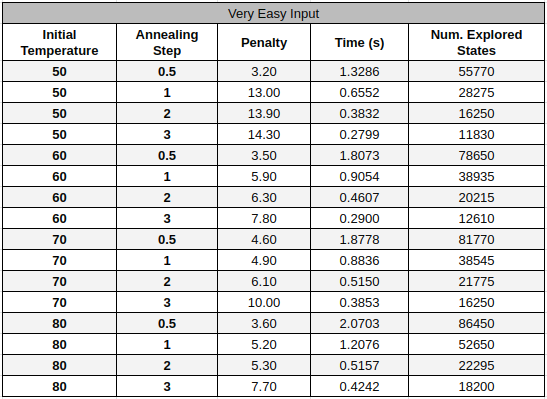
\includegraphics[width=250px]{annealing_very_easy.png}}
    \caption{Simulated Annealing Results on very easy inputs}
\end{figure}

\begin{figure}[H]
    \centerline{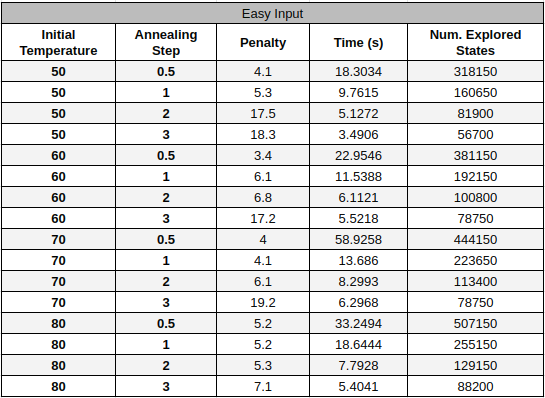
\includegraphics[width=250px]{annealing_easy.png}}
    \caption{Simulated Annealing Results on easy inputs}
\end{figure}

\begin{figure}[H]
    \centerline{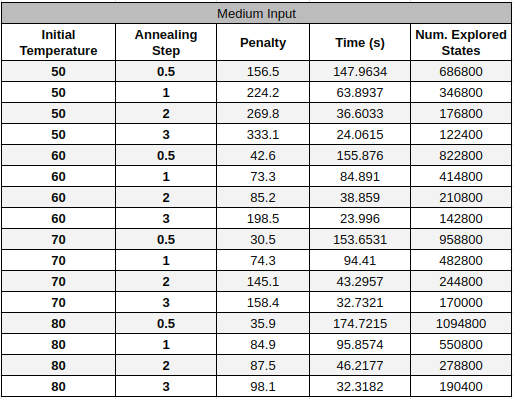
\includegraphics[width=250px]{annealing_medium.png}}
    \caption{Simulated Annealing Results on medium inputs}
\end{figure}

As expected, lower penalties (better solutions) were achieved with higher starting temperatures and lower annealing steps, since that results in more algorithm iterations. However, as the initial temperature increased and the annealing step decresed, the execution times and the number of explored states proportionally increased (as expected, since more algorithm iterations are being executed). These results were observed with inputs of all different difficulties.

\subsection{Genetic Algorithm Parameterizations}

The genetic algorithm makes use of three different parameterization variables: the generations population size, the mutation probability and the number of elite solutions preserved between consecutive generations. In order to understand which parameterizations achieve the best results, a set of 10 experiments with different parameterizations were made with inputs of different difficulties, with a maximum of 300 generations per experiment (may be less than this value if optimal is reached).

Firstly, the population size was manipulated (maintaining constant values for the other variables, namely a mutation probability of 15\% and a number of preserved elite solutions equal to 10\% of the population size). The obtained results were the following: 

\begin{figure}[H]
    \centerline{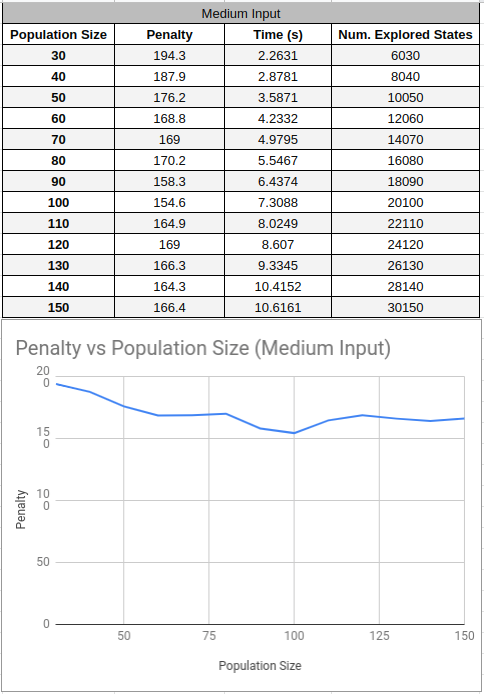
\includegraphics[width=250px]{genetic_pop_size_medium.png}}
    \caption{Genetic Algorithm Population size influence on medium inputs}
\end{figure}

As expected, the solution penalty decreased as the population size increased (since more solutions were explored and the different generations had more variability). The best performance was achieved, in all tested input difficulties, when the population size was approximately 100. The number of explored solutions and the execution time increased proportionally to the population size. 

Secondly, the mutation probability was manipulated (maintaining constant values for the other variables, namely a population size of 100 and a number of preserved elite solutions of 10). The obtained results were the following: 

\begin{figure}[H]
    \centerline{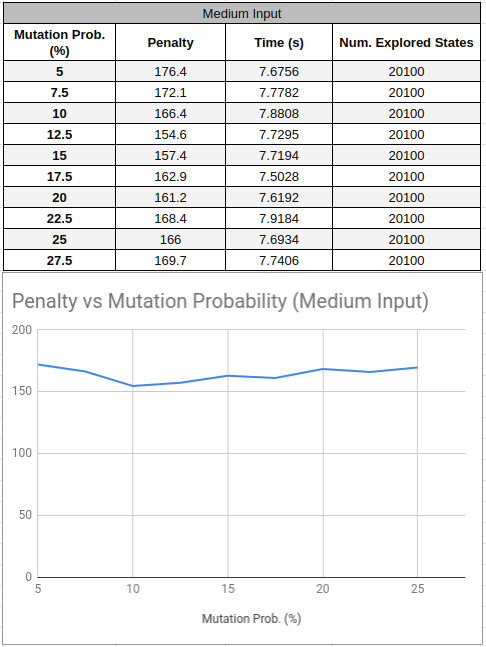
\includegraphics[width=250px]{mutation_prob_medium.png}}
    \caption{Genetic Algorithm Mutation Probability influence on medium inputs}
\end{figure}

The mutation probability did not have a significant impact on the solution's quality, although the algorithm achieved best performance with probabilities from 10\% to 15\% for all different input difficulties. The execution time and number of explored solutions were approximately independent (constant) of the different mutation probabilities.

Thirdly and finally, the number of preserved elite solutions between consecutive generations was manipulated (maintaining constant values for the other variables, namely a population size of 100 and a mutation probability of 12.5\%). The obtained results were the following: 

\begin{figure}[H]
    \centerline{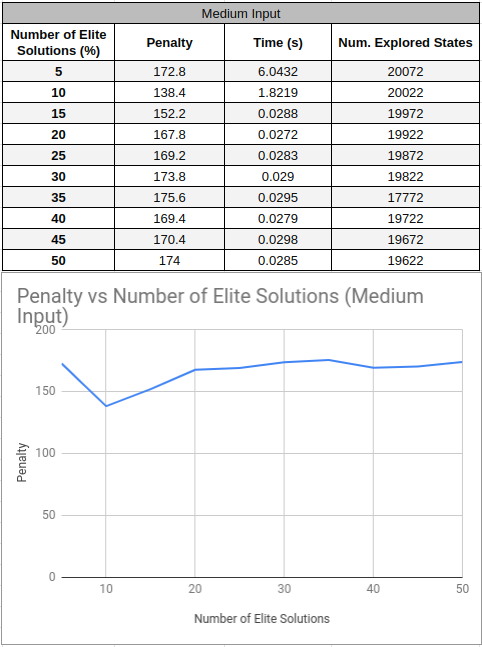
\includegraphics[width=250px]{elite_medium.png}}
    \caption{Genetic Algorithm number of Elite solutions influence on medium inputs}
\end{figure}

The best performance was achieved when the number of elite solutions was approximately 5\% to 10\% of the number of solutions in the population, for all different input difficulties. The number of explored solutions was approximately independant (constant) of the number of elite solutions. The execution time highly decreased as the number of elites increased, since there are less new solutions being generated for the new generation.

Based on the experiments, the optimal combination of parameterizations for the genetic algorithm are, approximately, 100 solutions in the generations population, maintaining 5\% to 10\% elite solutions between generations and with a mutation probability of 12.5\%.

\subsection{Algorithms Results and Comparison}

In order to study the algorithms performance with different difficulty inputs, all of the different inputs were tested, measuring the best achieved solution's penalty, the execution time and the number of explored solutions. The results were the following:  

\begin{figure}[H]
    \centerline{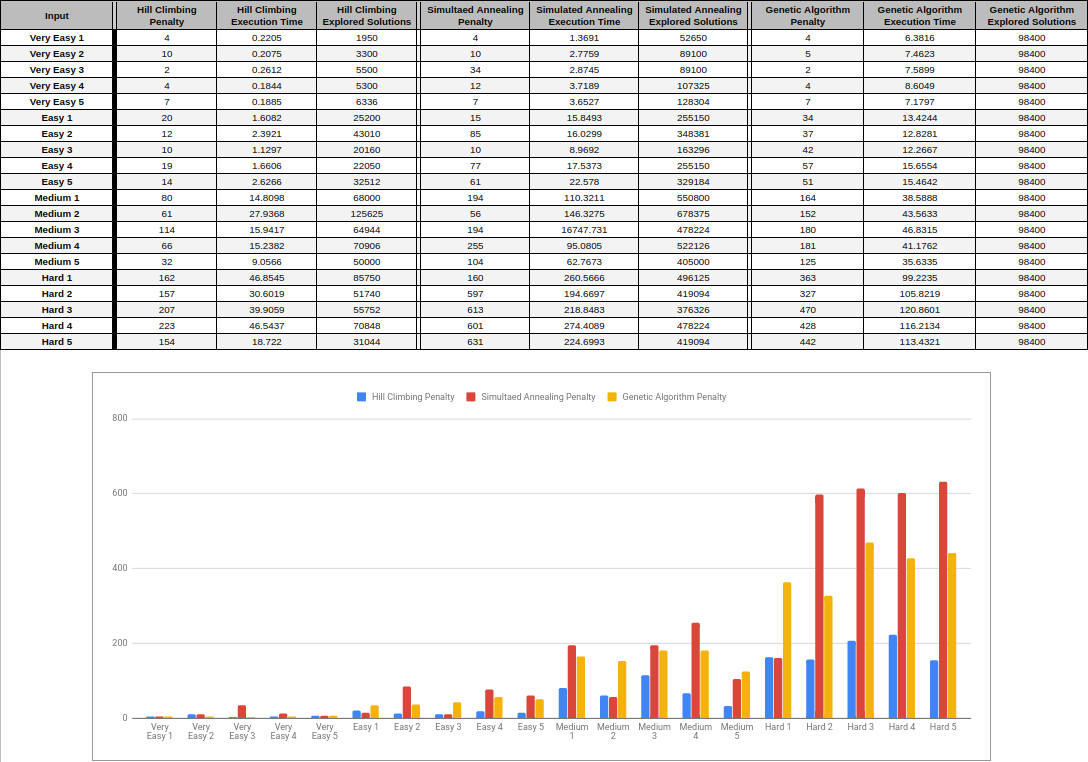
\includegraphics[width=255px]{comparison.png}}
    \caption{Optimization Algorithms comparison with different difficulty inputs}
\end{figure}

The results shown that the best performance was obtained by the Hill-Climbing algorithm, which achieved quality solutions (with low penalty) in very low execution times and without exploring a large number of solutions. This is verified due to the fact that, in this scheduling optimization problem, the local maximums that are quickly reached by the hill climbing algorithm have a high degree of quality (very low penalty, that is, low number of soft constraint violations). 

The full experiments results can be found in \autoref{sec:annex}.

\section{Conclusions and Future Work}

In this project, all of the applicable algorithms that were pro-posed were implemented and tested.

A command line interface was developed to test the different puzzles and visualize the solutions produced by each of the algorithms.

In order to study the upsides and downsides of each of the algorithms, a thorough examination of their performance using different metrics (produced solutions quality, execution time and number of explored solutions) was made. 

When analysing the produced solutions, it was concluded that the algorithm that achieved the overall best performance in the different difficulty inputs was the Hill Climbing algorithm (in terms of solution quality, execution time and number of explored solutions). 

All  of  the  objectives  were  successfully  completed  and future improvements could include the exploration of the studied algorithms performance in inputs of larger complexities.

\begin{thebibliography}{00}
    
\bibitem{air}{V. Ciesielski and P. Scerri, "Real time genetic scheduling of aircraft landing times," 1998 IEEE International Conference on Evolutionary Computation Proceedings. IEEE World Congress on Computational Intelligence (Cat. No.98TH8360), Anchorage, AK, USA, 1998, pp. 360-364.}

\bibitem{sol1}{Philipp Kostuch, "Timetabling Competition - SA-based Heuristic" in 1st International Timetabling Competition, January 2003.}

\bibitem{sol2}{Halvard Arntzen, Arne Lokketangen, "A local search heuristic for a university timetabling problem" in 1st International Timetabling Competition, January 2003}

\end{thebibliography}

\section{Annex} \label{sec:annex}

\subsection{Simulated Annealing metrics influence on Very Easy inputs}

\begin{figure}[H]
    \centerline{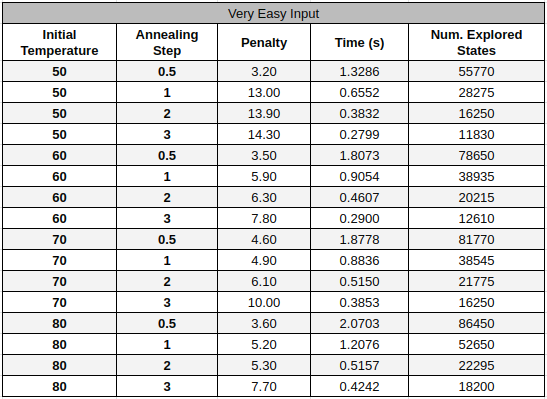
\includegraphics[width=250px]{annealing_very_easy.png}}
    \caption{Simulated Annealing metrics influence on Very Easy inputs}
\end{figure}

\subsection{Simulated Annealing metrics influence on Easy inputs}

\begin{figure}[H]
    \centerline{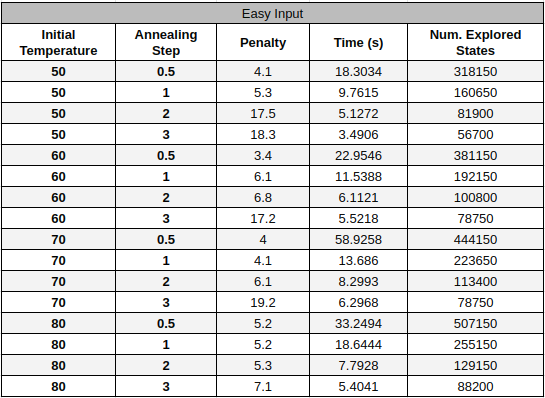
\includegraphics[width=250px]{annealing_easy.png}}
    \caption{Simulated Annealing metrics influence on Easy inputs}
\end{figure}

\subsection{Simulated Annealing metrics influence on Medium inputs}

\begin{figure}[H]
    \centerline{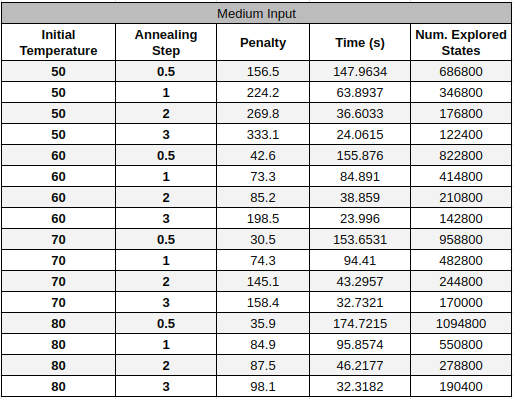
\includegraphics[width=250px]{annealing_medium.png}}
    \caption{Simulated Annealing metrics influence on Medium inputs}
\end{figure}

\subsection{Genetic Algorithms population size influence on Very Easy inputs}

\begin{figure}[H]
    \centerline{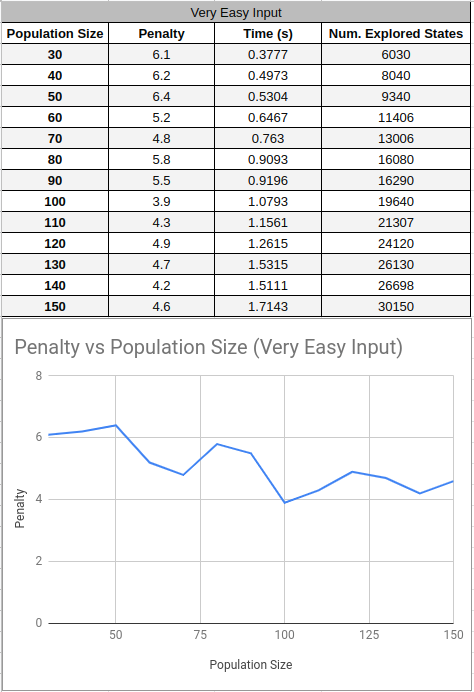
\includegraphics[width=250px]{genetic_pop_size_very_easy.png}}
    \caption{Genetic Algorithms population size influence on Very Easy inputs}
\end{figure}

\subsection{Genetic Algorithms population size influence on Easy inputs}

\begin{figure}[H]
    \centerline{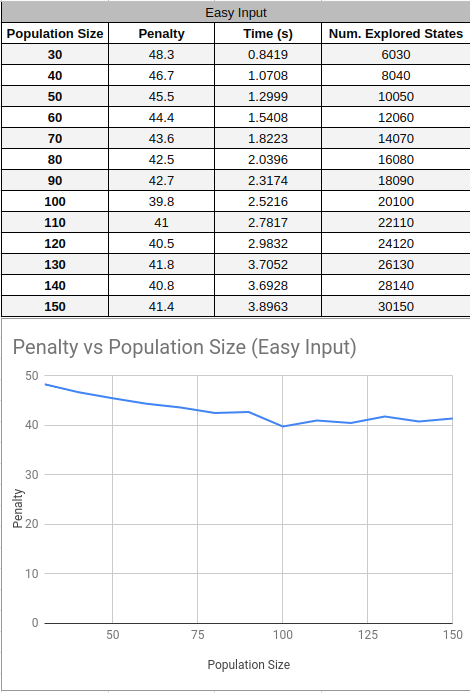
\includegraphics[width=250px]{genetic_pop_size_easy.png}}
    \caption{Genetic Algorithms population size influence on Easy inputs}
\end{figure}

\subsection{Genetic Algorithms population size influence on Medium inputs}

\begin{figure}[H]
    \centerline{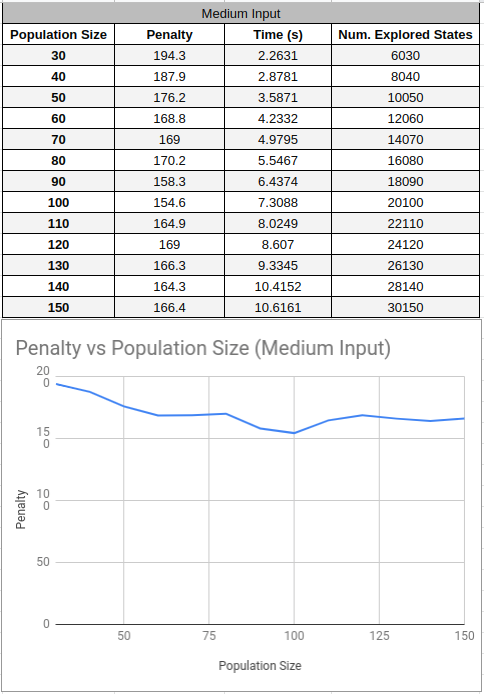
\includegraphics[width=250px]{genetic_pop_size_medium.png}}
    \caption{Genetic Algorithms population size influence on Medium inputs}
\end{figure}

\subsection{Genetic Algorithms population size influence on Hard inputs}

\begin{figure}[H]
    \centerline{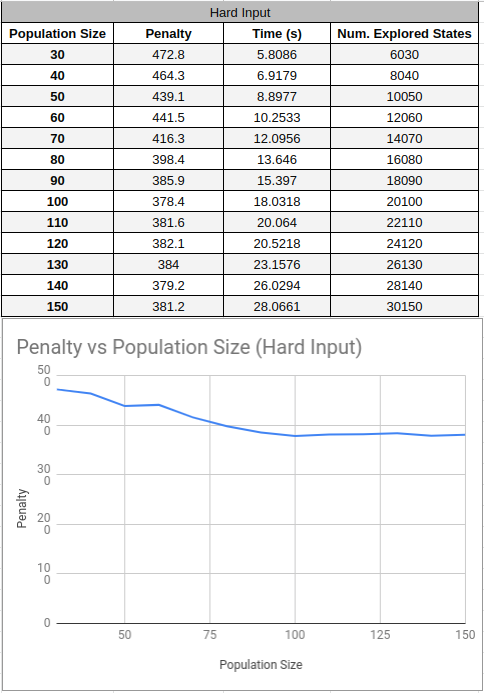
\includegraphics[width=250px]{genetic_pop_size_hard.png}}
    \caption{Genetic Algorithms population size influence on Hard inputs}
\end{figure}

\subsection{Genetic Algorithms mutation probability influence on Very Easy inputs}

\begin{figure}[H]
    \centerline{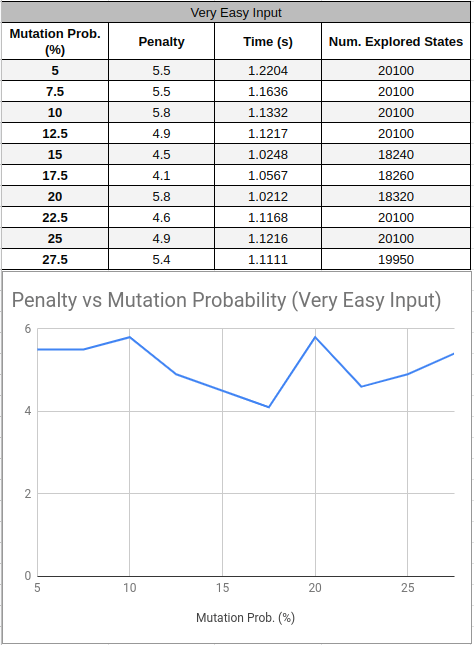
\includegraphics[width=250px]{mutation_prob_very_easy.png}}
    \caption{Genetic Algorithms mutation probability influence on Very Easy inputs}
\end{figure}

\subsection{Genetic Algorithms mutation probability influence on Easy inputs}

\begin{figure}[H]
    \centerline{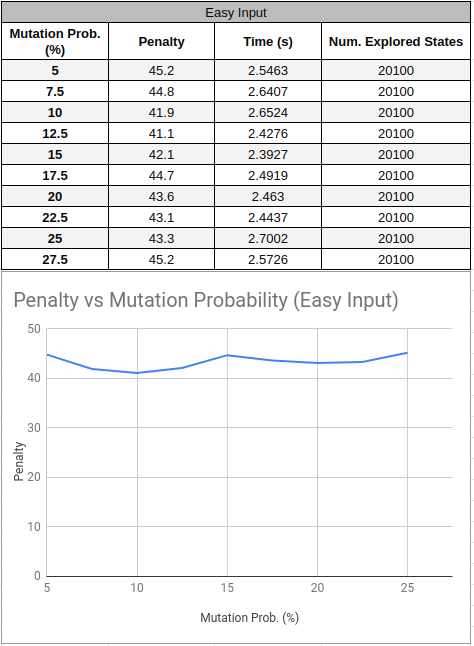
\includegraphics[width=250px]{mutation_prob_easy.png}}
    \caption{Genetic Algorithms mutation probability influence on Easy inputs}
\end{figure}

\subsection{Genetic Algorithms mutation probability influence on Medium inputs}

\begin{figure}[H]
    \centerline{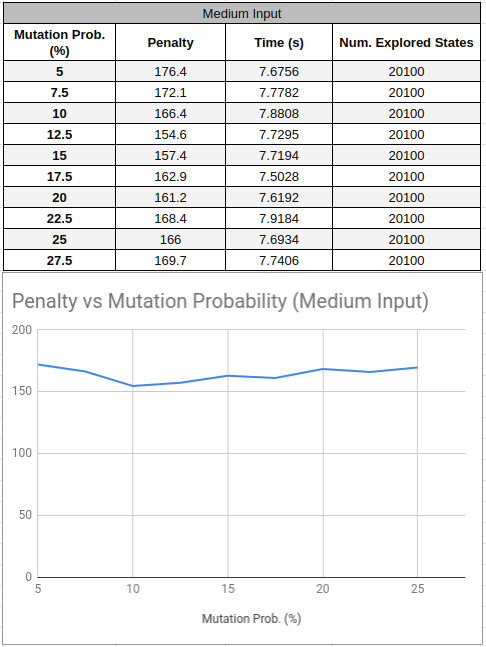
\includegraphics[width=250px]{mutation_prob_medium.png}}
    \caption{Genetic Algorithms mutation probability influence on Medium inputs}
\end{figure}

\subsection{Genetic Algorithms mutation probability influence on Hard inputs}

\begin{figure}[H]
    \centerline{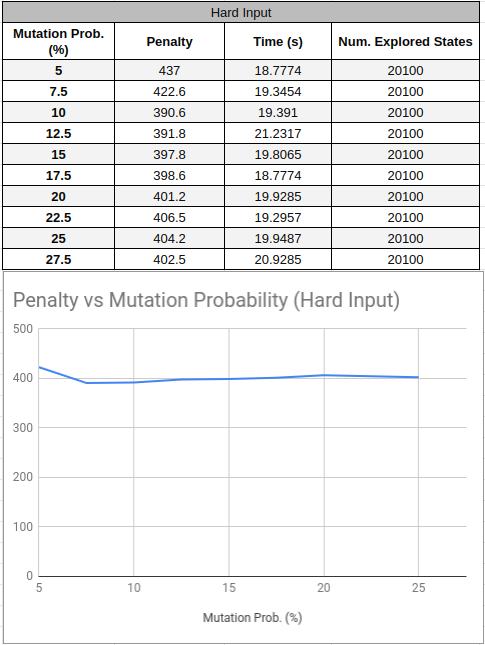
\includegraphics[width=250px]{mutation_prob_hard.png}}
    \caption{Genetic Algorithms mutation probability influence on Hard inputs}
\end{figure}

\subsection{Genetic Algorithms number of elite solutions influence on Very Easy inputs}

\begin{figure}[H]
    \centerline{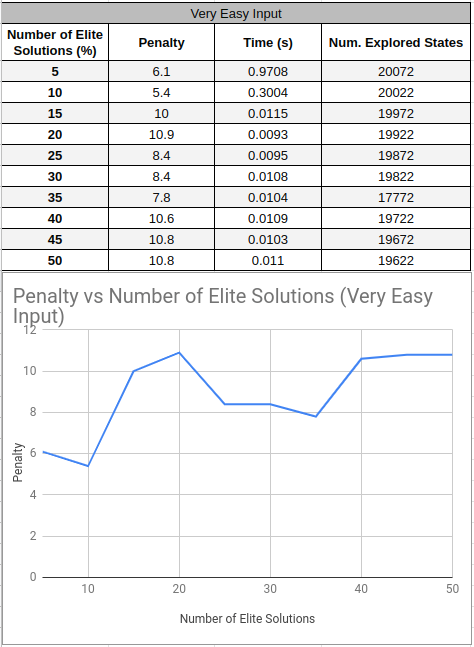
\includegraphics[width=250px]{elite_very_easy.png}}
    \caption{Genetic Algorithms number of elite solutions influence on Very Easy inputs}
\end{figure}

\subsection{Genetic Algorithms number of elite solutions influence on Easy inputs}

\begin{figure}[H]
    \centerline{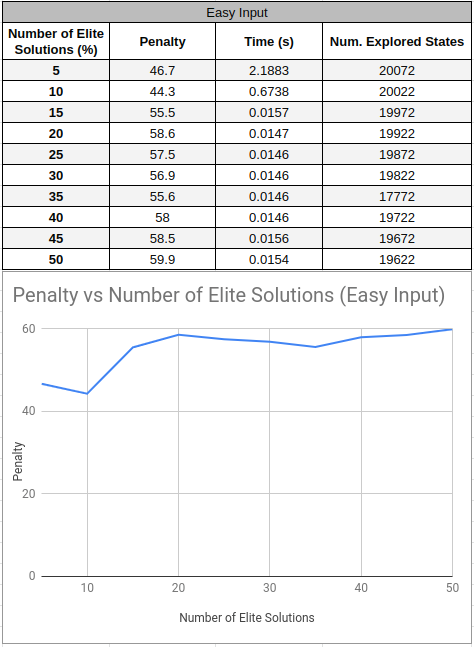
\includegraphics[width=250px]{elite_easy.png}}
    \caption{Genetic Algorithms number of elite solutions influence on Easy inputs}
\end{figure}

\subsection{Genetic Algorithms number of elite solutions influence on Medium inputs}

\begin{figure}[H]
    \centerline{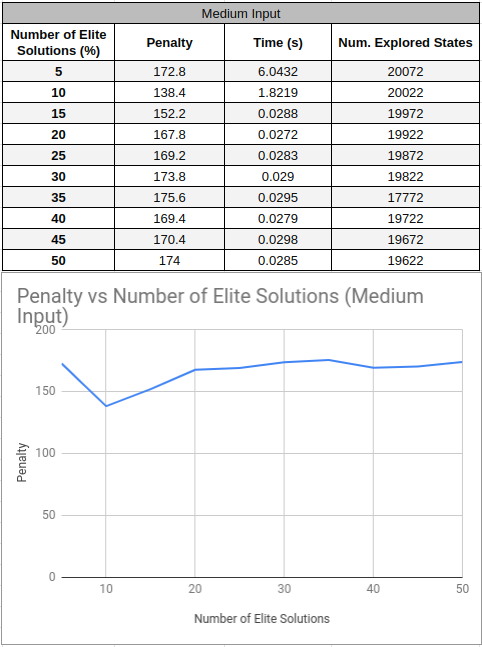
\includegraphics[width=250px]{elite_medium.png}}
    \caption{Genetic Algorithms number of elite solutions influence on Medium inputs}
\end{figure}

\subsection{Genetic Algorithms number of elite solutions influence on Hard inputs}

\begin{figure}[H]
    \centerline{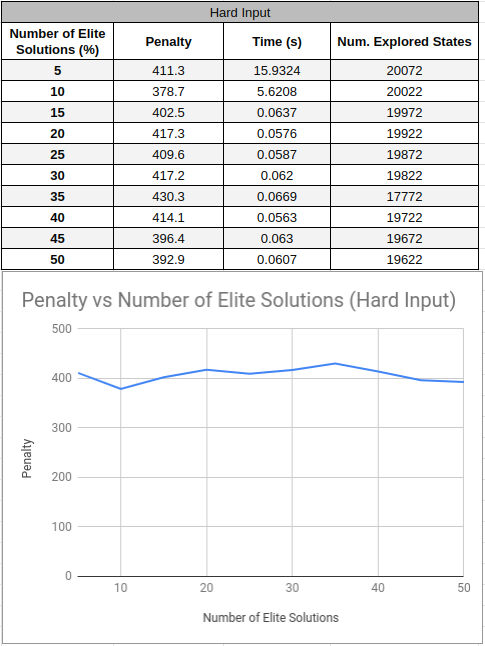
\includegraphics[width=250px]{elite_hard.png}}
    \caption{Genetic Algorithms number of elite solutions influence on Hard inputs}
\end{figure}

\subsection{Algorithms performance comparison on different difficulty inputs}

\begin{figure}[H]
    \centerline{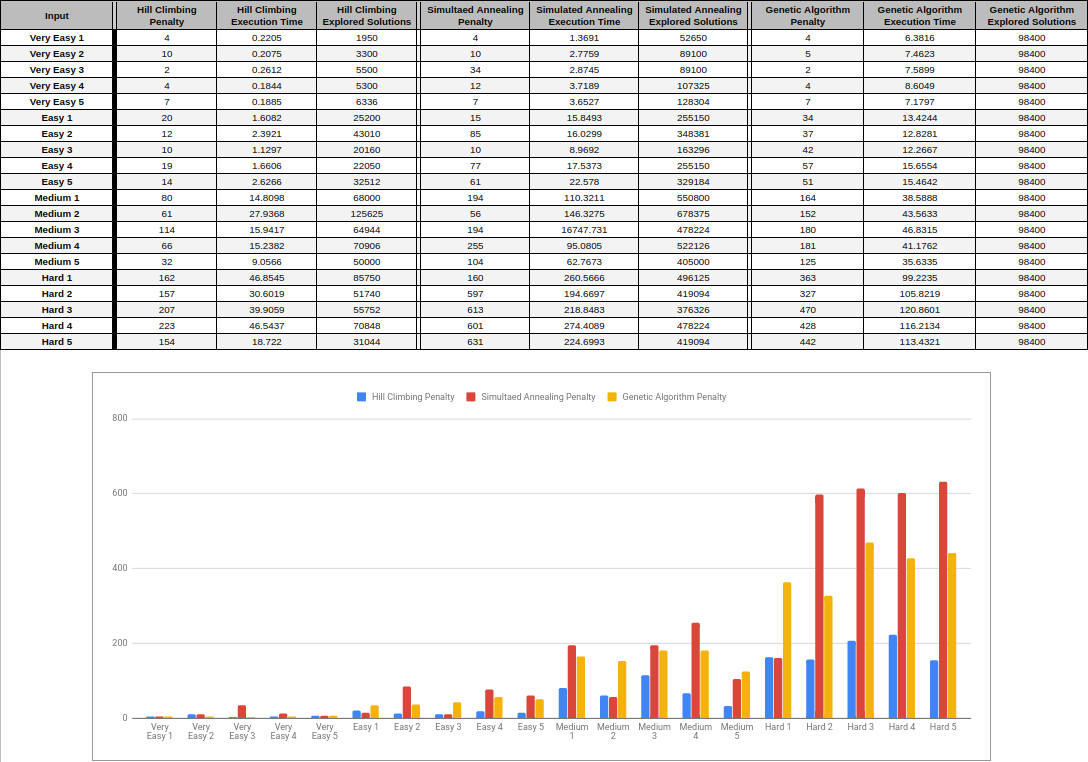
\includegraphics[width=250px]{comparison.png}}
    \caption{Algorithms performance comparison on different difficulty inputs}
\end{figure}

\end{document}
